\section{Koncepce}

V následující kapitole je definován konceptuální model\footnote{\url{https://www.fit.vutbr.cz/study/courses/IMS/public/prednasky/IMS.pdf}, slide 48}, který jsme vytvořili na základě faktů systému představených v předcházející kapitole. Na základě konceptuálního modelu jsme následně vytvořili model simulační\footnote{\url{https://www.fit.vutbr.cz/study/courses/IMS/public/prednasky/IMS.pdf}, slide 44}.



\subsection{Způsob vyjádření konceptuálního modelu}

Následující schéma prezentuje systém jako celek. Tento systém budeme dále dělit na podsystémy a modelovat pomocí Petriho sítí\footnote{\url{https://www.fit.vutbr.cz/study/courses/IMS/public/prednasky/IMS.pdf}, slide 123}.

\begin{figure}[H]
    \centering
    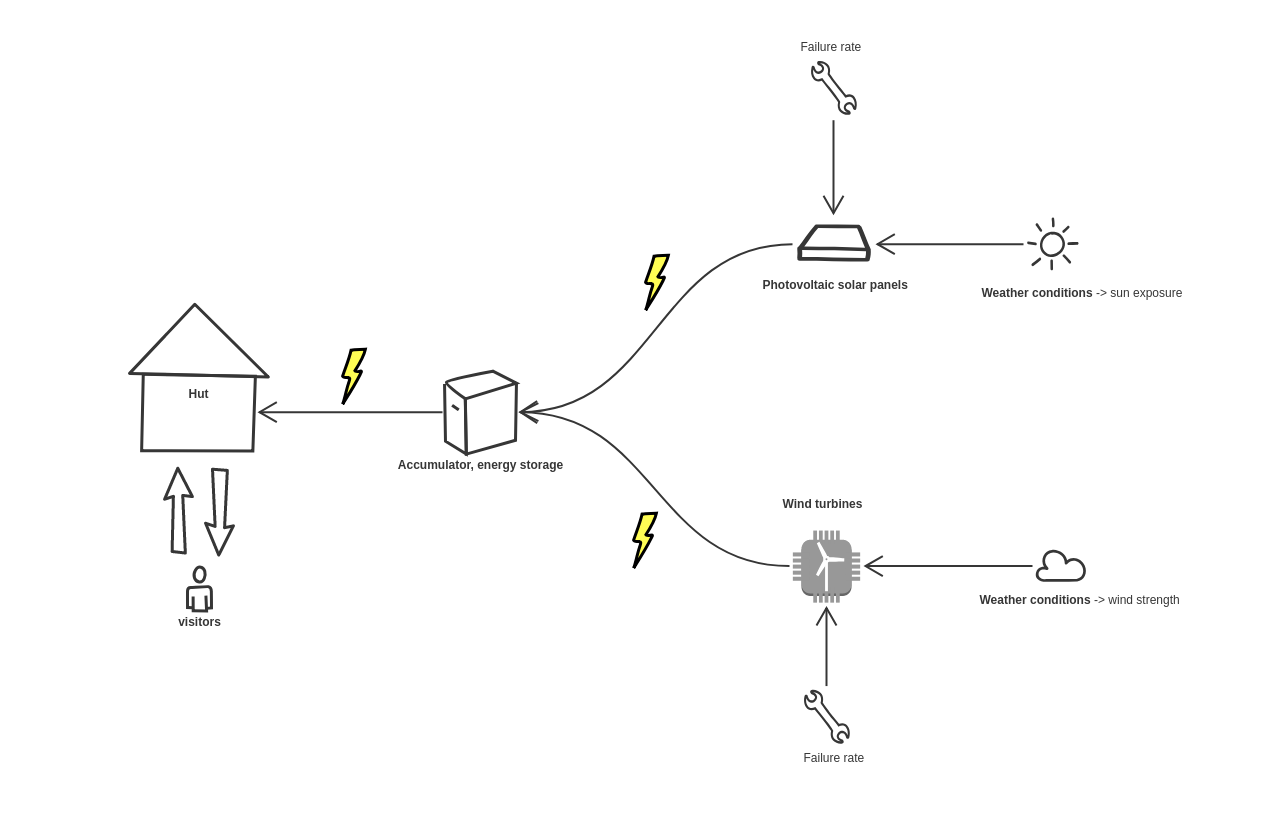
\includegraphics[width=.99\textwidth]{images/schema.png}\hfill
    \caption{Schéma systému}
    \label{fig:schema}
\end{figure}



\subsection{Forma konceptuálního modelu}

Na dalších obrázcích jsou zachyceny jednotlivé podsystémy modelované Petriho sítí.

\begin{figure}[H]
    \centering
    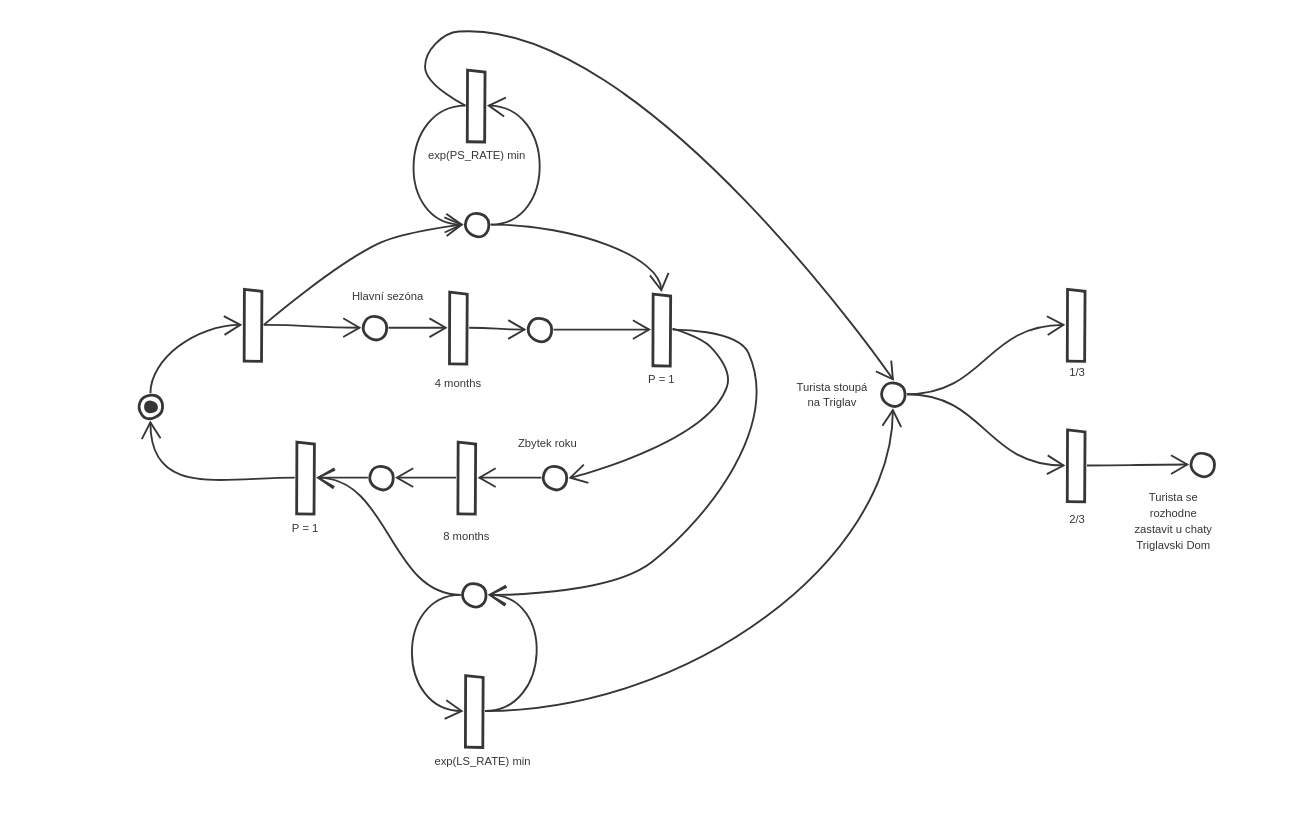
\includegraphics[width=.99\textwidth]{images/petri_net_visitors.png}\hfill
    \caption{Generování turistů}
    \label{fig:petri_net_visitors}
\end{figure}

\begin{figure}[H]
    \centering
    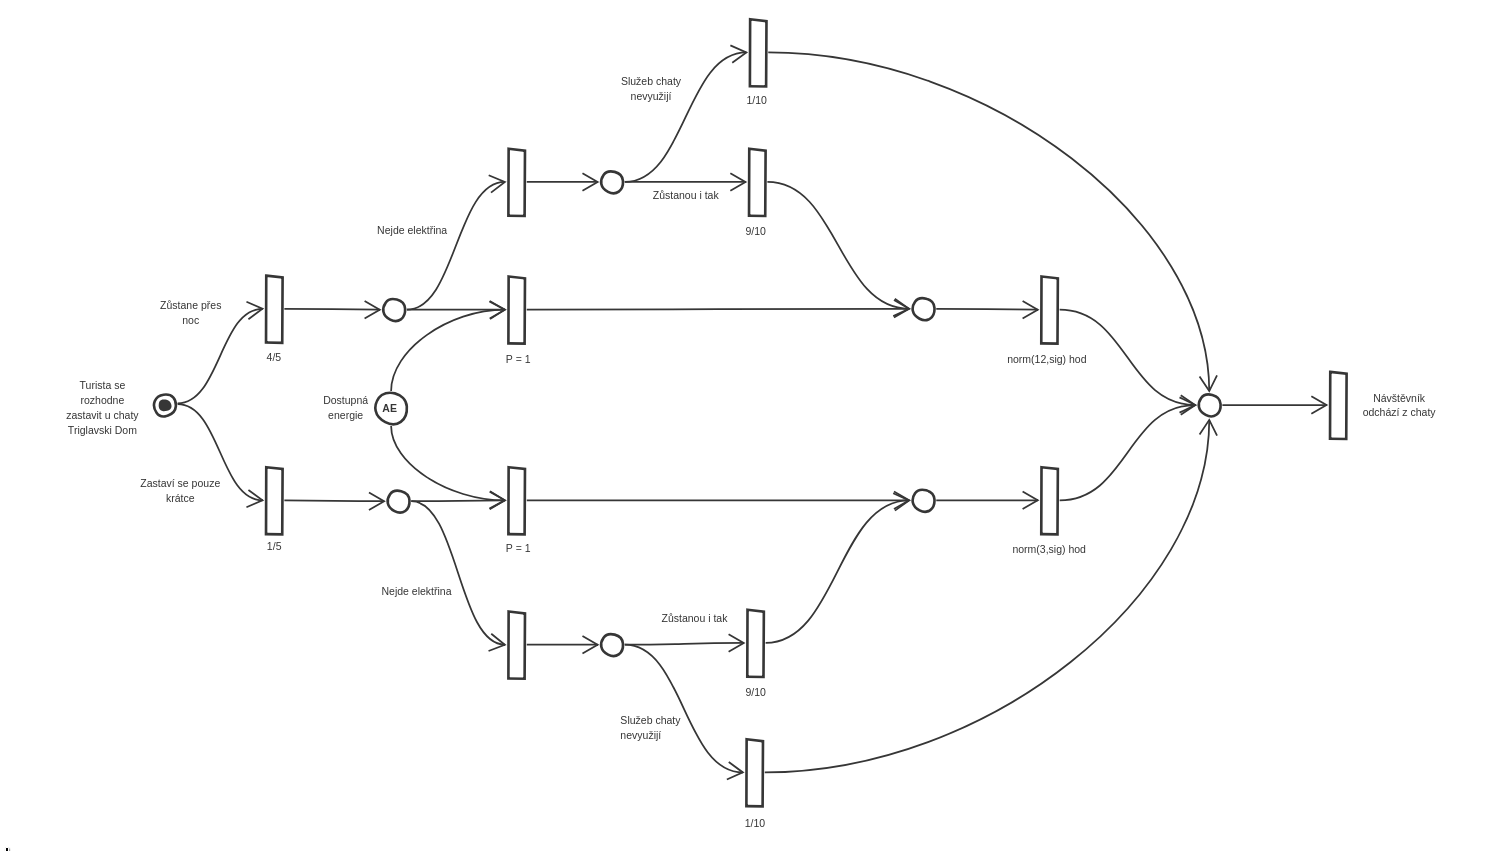
\includegraphics[width=.99\textwidth]{images/petri_net_visitor_in_hut.png}\hfill
    \caption{Návštěvník v chatě}
    \label{fig:petri_net_visitor_in_hut}
\end{figure}

\begin{figure}[H]
    \centering
    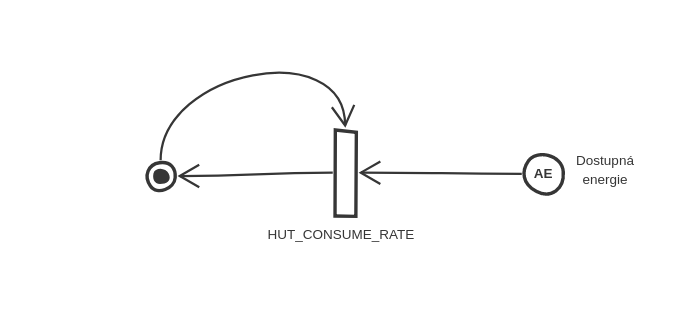
\includegraphics[width=.5\textwidth]{images/petri_net_hut.png}\hfill
    \caption{Energie potřebná pro základní chod chaty}
    \label{fig:petri_net_hut}
\end{figure}

\begin{figure}[H]
    \centering
    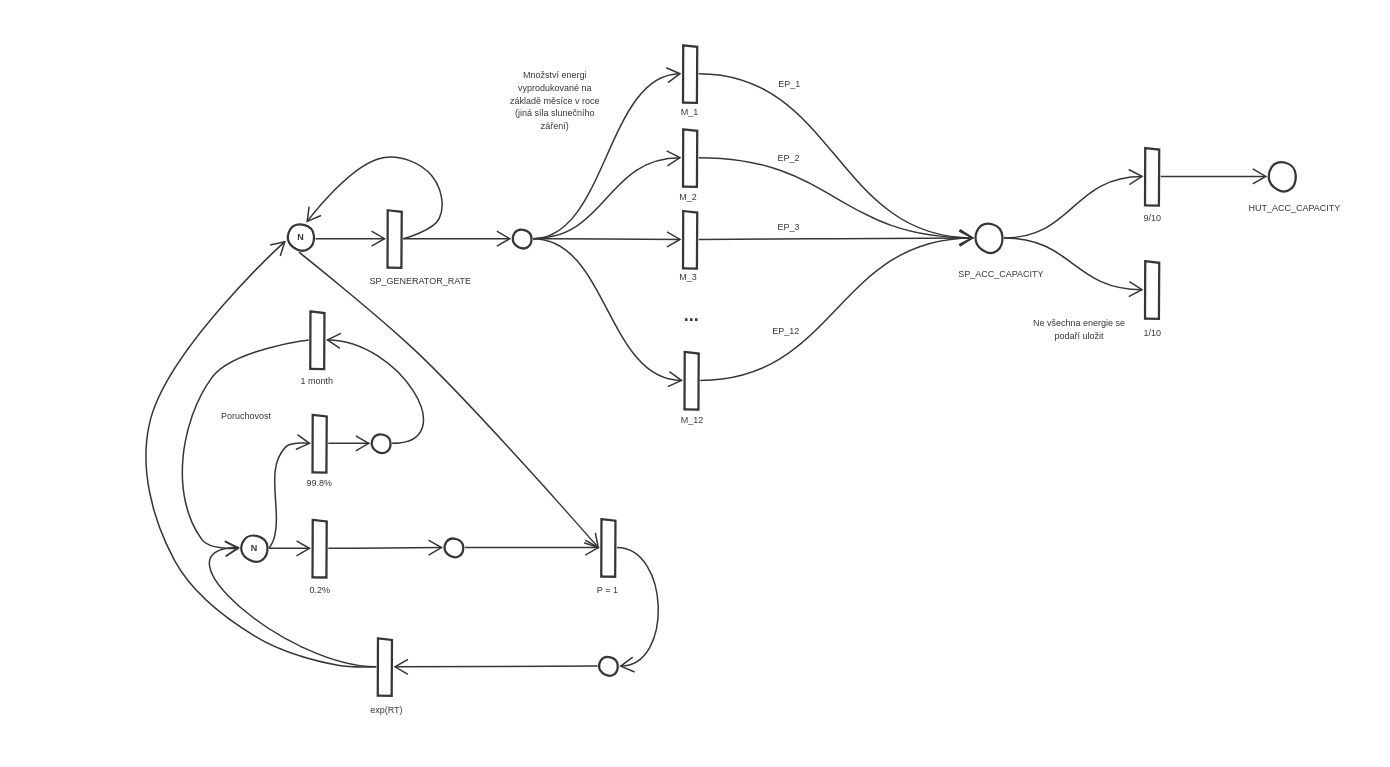
\includegraphics[width=.99\textwidth]{images/petri_net_solar_energy.png}\hfill
    \caption{Energie generovaná solárními panely}
    \label{fig:petri_net_solar_energy}
\end{figure}

\begin{figure}[H]
    \centering
    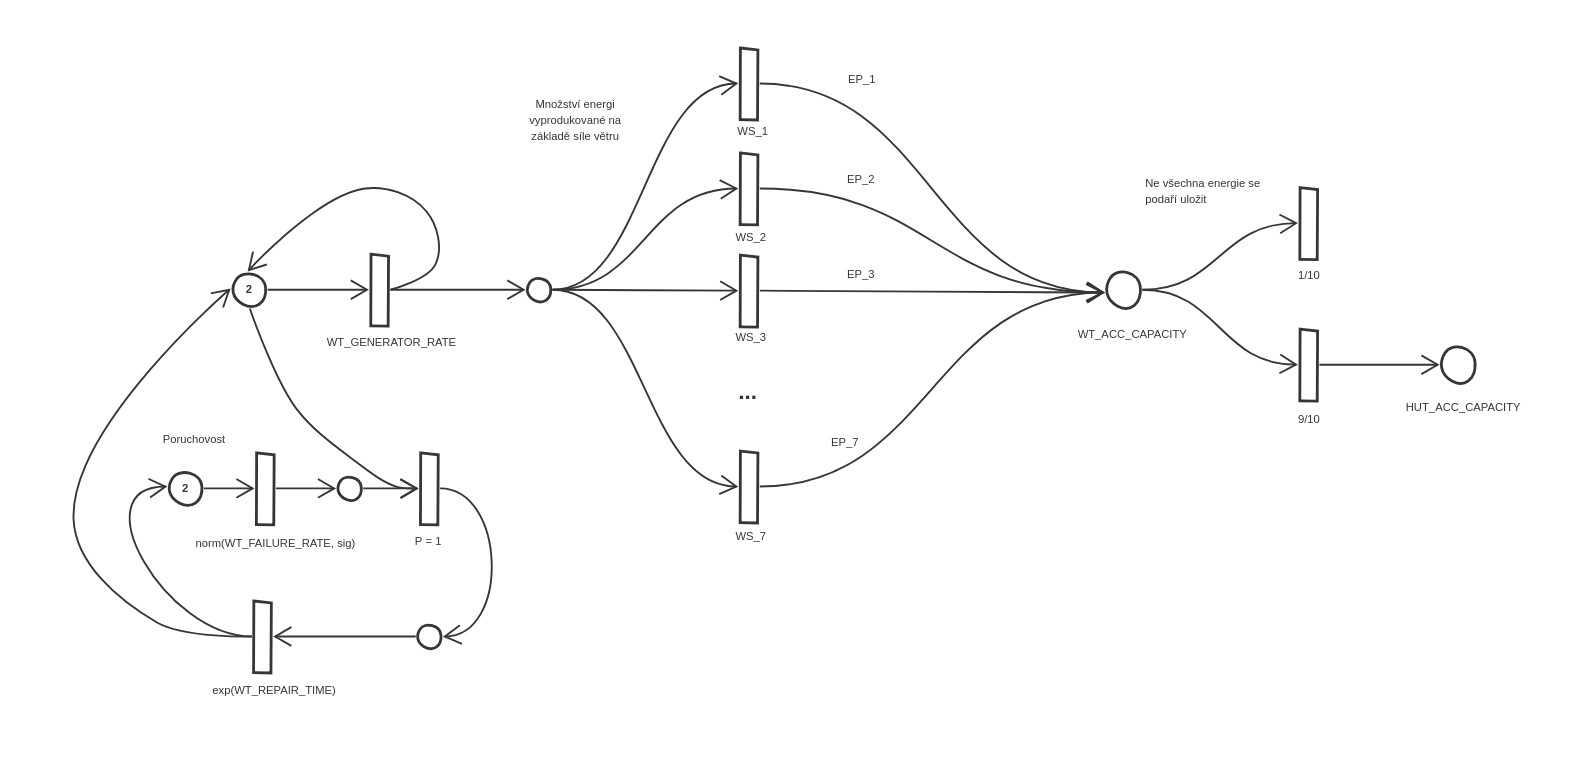
\includegraphics[width=.99\textwidth]{images/petri_net_wind_energy.png}\hfill
    \caption{Energie generovaná větrnými turbínami}
    \label{fig:petri_net_wind_energy}
\end{figure}
